\documentclass[letterpaper,12pt]{article}
\usepackage[latin1]{inputenc}
\usepackage[dvips]{graphicx}
\usepackage[spanish]{babel}
\usepackage{graphicx}
\usepackage[fleqn]{amsmath}
\usepackage{amssymb}
\usepackage{amsmath}
\usepackage{fullpage}
\newcommand{\eq}[1]{\begin{align}#1\end{align}}
%opening
\title{Ejercicios de \emph{Classical Mechanics} de H. Goldstein}
\author{Nicol\'as Quesada M. \\ {\small \sf Instituto de F\'isica, Universidad de Antioquia}}
\date{}
\begin{document}

\maketitle
\section*{Cap\'itulo 1}



\subsection*{Ejercicio 1.6.}
Supongamos que en alg\'un instante $t$ la part\'icula tiene coordenadas $(x',y')$ y que la tangente del \'angulo que forma su velocidad con el eje $x$ esta dada por $\frac{dy(t)}{dx(t)}$. La recta tangente a la curva estar\'a dada por:
\eq{
(y-y')=\frac{dy(t)}{dx(t)} (x-x').
}
Por otro lado seg\'un el problema la velocidad siempre debe apuntar a un punto en el eje $x$, al que llamaremos $f(t)$. Pero este punto no es m\'as que el intercepto con el eje $x$ de la recta anteriormente definida. As\'i entonces debemos tener lo siguiente:
\eq{
-y'&=\frac{dy(t)}{dx(t)} (f(t)-x')\\
(f(t)-x)dy+y dx&=0
}
Que es la ecuaci\'on de una ligadura no-hol\'onoma. Para mostrar que la ligadura es no hol\'onoma se trata de buscar un factor integrante para obtener una diferencial total:
\eq{
dF=f_i(f(t)-x)dy+ f_i y dx+f_i \times 0 dt.
}
De aqu\'i se lee que:
\eq{
\frac{\partial F}{\partial y}&=f_i(f(t)-x) \\
\frac{\partial F}{\partial x}&= f_i y\\
\frac{\partial F}{\partial t}&=0.
}
Haciendo derivadas cruzadas entre $x$ y $t$ 
(y teniendo en cuenta que $x$ y $y$ dependen de $t$ s\'olo impl\'icitamente):
\eq{
\frac{\partial \left(\frac{\partial f_i}{\partial x}\right)}{\partial t}=y \frac{\partial f_i}{\partial t}
=0.
}
Tomando derivadas cruzadas de $t$ y $y$ nos queda que:
\eq{
 0=\frac{\partial \left(\frac{\partial F}{\partial y}\right)}{\partial t}=f_i \frac{\partial f(t)}{\partial t}=0
}
Asi o bien $f_i=0$ o $f(t)=cte$, pero lo anterior va encontra de las hip\'otesis ya que $f(t)$ es arbitrario.


\subsection*{Ejercicio 1.9 }
Tenemos que el Lagrangiano para una part\'icula en presencia de un campo El\'ectrico 
$\vec E=\nabla \phi -\frac{\partial \vec A}{\partial t}$
y un campo magn\'etico  $\vec B=\nabla \times \vec A$ est\'a dado por 
\eq{
L = {1 \over 2} m \vec{v} \cdot \vec{v}  - q\phi + {q \over c} \vec{v} \cdot \vec{A} .
}
Se pregunta que efecto tiene sobre el lagrangiano el cambiar el potencial escalar $\phi$ y el potencial vectorial $\vec A$ 
\eq{
\vec A &\longmapsto \vec A+\nabla \psi \\
\phi &\longmapsto \phi-\frac{1}{c}\frac{\partial \psi}{\partial t}
}
sobre el Lagrangiano y las ecuaciones de movimiento de la part\'icula sobre la que act\'uan $\vec E$ y $\vec B$, siendo $\psi(x,y,z,t)$ una funci\'on arbitraria pero diferenciable.
Si sustituimos en el Lagrangiano y reorganizamos t\'erminos se obtiene lo siguiente:
\eq{
 L' =&{1 \over 2} m \vec{v} \cdot \vec{v} -q \left(\phi-\frac{1}{c}\frac{\partial \psi}{\partial t}\right)+\frac{q}{c}\vec v \cdot  \left(\vec A+\nabla \psi\right)\\
 L'=&\left({1 \over 2} m \vec{v} \cdot \vec{v}-q \phi+\frac{q}{c}\vec v \cdot  \vec A\right)+\frac{q}{c}\left(\frac{\partial \psi}{\partial t}+\vec v \cdot \nabla \psi\right)
}
El t\'ermino dentro del par\'entesis es el lagrangiano original $L$ y el segundo es la diferencial total  de $\psi$ con respecto a $t$:
\eq{
\frac{d \psi}{dt}=\frac{\partial \psi}{\partial x}\frac{dx}{dt}+\frac{\partial \psi}{\partial y}\frac{dy}{dt}+\frac{\partial \psi}{\partial z}\frac{dz}{dt}+\frac{\partial \psi}{\partial t}=\nabla \psi \cdot \vec v+\frac{\partial \psi}{\partial t}
}
Asi entonces $L'$ se reescribe como $L$ mas la derivada total con respecto a $t$ de una funci\'on arbitraria $\psi$:
\eq{
L'=L+\frac{d \psi}{dt}
}
Pero seg\'un la demostraci\'on 8 Las ecuaciones de Lagrange se siguen satisfaciendo si a un Lagrangiano $L$ se le adiciona la derivada total con respecto al tiempo de una funci\'on arbitraria $\psi$, es decir las ecuaciones de movimiento de la part\'icula no cambian.


\subsection*{Ejercicio 1.19}
Usando coordenadas esf\'ericas y teniendo en cuenta que el p\'endulo es inextensible tenemos que la velocidad se puede escribir as\'i:
\eq{
\vec v=\frac{d\vec r}{dt}=\frac{dr}{dt}\hat r+r\frac{d\theta}{dt}\hat \theta+r \sin \theta \frac{d\phi}{dt} \hat \phi=r\frac{d\theta}{dt}\hat \theta+r \sin \theta \frac{d\phi}{dt} \hat \phi
}
y que el potencial gravitacional se puede escribir como (con $z$ positivo hacia abajo):
\eq{
V=-mgz=-mgr \cos \theta
}
Asi el Lagrangiano del sistema es:
\eq{
L&=\frac{1}{2} m r^2 \left(\sin ^2(\phi ) \dot \theta^2+\dot \phi^2\right) +mgr \cos (\phi ) \\
\frac{\partial L}{\partial \dot \theta}&=m r^2 \dot \theta\\
\frac{\partial L}{\partial \dot \phi}&=m r^2 \sin^2\theta \dot \phi\\
\frac{\partial L}{\partial \theta}&=m r^2 \sin \theta \cos \theta \dot \phi^2-m g r \sin \theta\\
\frac{\partial L}{\partial \phi}&=0
}
luego las ecuaciones de movimiento son:
\eq{
m r^2 \sin \theta \cos \theta \dot \phi^2-m g r \sin \theta-m r^2 \frac{d\dot \theta}{dt}=0\\
\frac{d }{dt}\left( m r^2 \sin^2\theta \dot \phi\right)=0
}



\section*{Cap\'itulo 2}
\documentclass[letterpaper,10pt]{article}
\usepackage[dvips]{graphicx}
\usepackage[spanish]{babel}


\textwidth = 16.5 cm
\textheight = 23.5 cm
\oddsidemargin = 0.0 cm
\evensidemargin = 0.0 cm
\topmargin = 0.0 cm
\headheight = 0.0 cm
\headsep = 0.0 cm 

\title{Ejercicios del cap\'itulo 2 de\\ \emph{Classical Mechanics} de H. Goldstein}
\author{Nicol\'as Quesada M. \\ {\small \sf Instituto de F\'isica, Universidad de Antioquia}}
\date{}

\begin{document}
\maketitle
\section*{Ejercicio 2.1}
En el problema de la braqu\'istocrona, se llega a que se debe minizar el funcional
\begin{eqnarray}
\label{integ}
 S&=&\int_1^2 \sqrt{\frac{1+y'(x)^2}{ 2g y(x)}}dx\\
f&=&\sqrt{\frac{1+y'(x)^2}{ 2g y(x)}}.
\end{eqnarray}
La ecuaci\'on de Euler-Lagrange para el problema se obtiene facilmente haciendo los siguientes c\'alculos:
\begin{eqnarray}
\frac{\partial f}{\partial y'(x)}&=&\frac{y'(x)}{\sqrt{(2 g y(x))(1+y'(x)^2)}}\\
\frac{\partial f}{\partial y(x)}&=&\frac{\sqrt{1+y'(x)^2}}{2 y \sqrt{2 g y}}\\
0=\frac{d\left(\frac{\partial f}{\partial y'(x)} \right)}{dx}-\frac{\partial f}{\partial y(x)}&=&\frac{d\left( \frac{y'(x)}{\sqrt{(2 g y(x))(1+y'(x)^2)}}\right)}{dx}-\frac{\sqrt{1+y'(x)^2}}{2 y \sqrt{2 g y}}=-\frac{y'(x)^2+2 y(x) y''(x)+1}{2 \sqrt{2} g^2 y(x)^3
   \left(\frac{y'(x)^2+1}{g y(x)}\right)^{3/2}} .
\end{eqnarray}
La ecuaci\'on diferencial que debemos resolver es entonces:
\begin{equation}
y'(x)^2+2 y(x) y''(x)+1=0.
\label{n}
\end{equation}
Podemos notar que $f$ no depende explictamente de $x$, entonces la cantidad $h=\frac{\partial f}{\partial y'(x)}y'(x)-f$ es una cantidad conservada. Para este caso $h$ tiene la siguiente forma:
\begin{eqnarray}
h&=&-\frac{1}{\sqrt{2 g y(x)(1+y'(x)^2)}}=cte \\
\frac{1}{h^2}&=&2 g y(x) (1+y'(x))^2.
\end{eqnarray}
Si se deriva la \'ultima de las ecuaciones con respecto a $x$ se llega a :
\begin{eqnarray}
0= \frac{d \left(\frac{1}{h^2}\right)}{dx}=g y'(x) \left(y'(x)^2+1\right)+2 g y(x) y'(x) y''(x)
\end{eqnarray}
Que es la misma ecuaci\'on (\ref{n}) multiplicada por $g y'(x)$. Es decir la ecuaci\'on (\ref{n}) es equivalente a $y(x) (1+y'(x)^2)=2c$. De esta ecuaci\'on se puede despejar $y'(x)$ separar variables e integrar para obtener :
\begin{eqnarray}
 y'(x)^2&=&\frac{2c}{y}-1\\
\frac{dy}{\sqrt{\frac{2c}{y}-1}}&=&dx\\
 2 c \tan ^{-1}\left(\frac{1}{\sqrt{\frac{2
   c}{y}-1}}\right)-\sqrt{(2 c-y) y}  &=&x.
\end{eqnarray}
Pero $\tan^{-1}(x)=\cos^{-1}(\frac{1}{\sqrt{1+x^2}})$ entonces:
\begin{eqnarray}
2 c \cos ^{-1}\left(\sqrt{1-\frac{y}{2
   c}}\right)-\sqrt{(2 c-y) y}=x\\
1-\frac{y}{2c}=\cos^2\left(\frac{x+\sqrt{y(2c-y)}}{2c}\right).
\end{eqnarray}
Llamando $\alpha=\frac{x+\sqrt{y(2c-y)}}{c}$ y despejando:
\begin{eqnarray}
\frac{y}{2c}=1-\cos^2\left(\frac{\alpha}{2}\right)=\frac{1-\cos(\alpha)}{2}\\
\frac{y}{c}=1-\cos\left(\frac{x+\sqrt{y(2c-y)}}{c} \right)
\end{eqnarray}
La \'ultima igualdad se obtiene de las identidades de \'angulo mitad para el coseno.
De esta igualdad tambien se ve que $y$ s\'olo puede tomar valores en el intervalo $[0,2a]$ (ya que la que la cantidad dentro del radical del coseno s\'olo es mayor que 0 en este intervalo) y que uno de sus m\'inimos est\'a en $(0,0)$(que fue de donde se lanz\'o la part\'icula), es decir all\'i hay una c\'uspide.\\
Por otro lado para mostrar que si la part\'icula se proyecta con una energia cin\'etica inicial $\frac{1}{2}m v_0^2$ entonces tambien est\'a se mueve sobre un cicloide basta notar que la integral (\ref{integ}) se reescribe de esta forma (Conservaci\'on de Energia: $\frac{1}{2}m v_0^2=\frac{1}{2} mv^2-mgy$):
\begin{eqnarray}
S=\int_1^2 \sqrt{\frac{1+y'(x)^2}{2 g y(x)+v_0^2}}dx
\end{eqnarray}

Esta puede ser devuelta a su forma original haciendo el cambio de variable $\hat y=y+\frac{v_0^2}{2g}$, esto equivale a mover el sistema de coordenadas $\frac{v_0^2}{2g}$ unidades, por lo tanto la c\'uspide que estaba en $y=0$ quedar\'a $\frac{v_0^2}{2g}$ unidades mas arriba.


\section*{Ejercicio 2.3 }
La soluci\'on a este problema es minimizar el funcional $$J=\int_1^2 \sqrt{dx^2+dy_1^2+dy_2^2}=\int_{x_1}^{x_2} \sqrt{1+\left(\frac{dy_1}{dx}\right)^2+\left(\frac{dy_2}{dx}\right)^2}dx$$, para esto resolvemos:
\begin{eqnarray}
\label{eu}
\frac{\partial f}{\partial y_i}-\frac{d\left(\frac{\partial f}{\partial \dot y_i}\right)}{dx}=0
\end{eqnarray}
\begin{eqnarray}
f=\sqrt{1+\dot y_1^2+\dot y_2^2}\\
\dot y_i=\frac{dy_i}{dx},
\end{eqnarray}
con $f$ as\'i definida obtenemos:
\begin{eqnarray}
 \frac{\partial f}{\partial y_i}=0\\
\frac{\partial f}{\partial \dot y_i}=\frac{\dot y_1}{\sqrt{1+\sum_i\dot y_i^2}}.\\
\end{eqnarray}
as\'i llegamos a que:
\begin{eqnarray}
\frac{d}{dx}\left(\frac{\dot y_i}{\sqrt{1+\sum_i\dot y_i^2}}\right)=0\\
\frac{\dot y_i}{\sqrt{1+\sum_i\dot y_i^2}}=c_i.
\end{eqnarray}
La \'ultima ecuaci\'on se puede solucionar para las $y_i$:
\begin{eqnarray}
\dot y_i^2= \frac{c_i^2}{1-\sum_i c_i}
\end{eqnarray}
y finalmente:
\begin{eqnarray}
y_i=a_i x +b_i
\end{eqnarray}
Las anteriores son las ecuaciones de una recta parametrizadas por la primera de sus coordenadas.

\section*{Ejercicio 2.4 }
Con un procedimiento an\'alogo al anterior pero usando coordenadas polares $(r,\theta,\phi)$ (con $r$ fijo) llegamos a que $ds^2=r^2(d\theta^2+\sin^2 \theta d\phi^2) $ llegamos al siguiente funcional
\begin{equation}
 F=\int_1^2 \sqrt{d\theta^2+\sin^2\theta d\phi^2}=\int_{\theta_1}^{\theta_2}{\sqrt{1+\sin^2\theta (\frac{d\phi}{d\theta})^2} d\theta}.
\end{equation}
Haciendo uso de (\ref{eu}) pero con $f=\sqrt{1+\sin^2\theta (\frac{d\phi}{d\theta})^2}$ , $y_i=\phi$ , $x=\theta$ y $\dot \phi=\frac{d\phi}{d\theta}$
obtenemos lo siguiente:
\begin{eqnarray}
\frac{\partial f}{\partial \phi}=0\\
\frac{\partial f}{d\dot \phi}=\frac{\sin^2 \theta \dot \phi}{\sqrt{1+\sin^2 \theta  \dot \phi^2}}\\
\frac{d \left(\frac{\sin^2 \theta \dot \phi}{\sqrt{1+\sin^2 \theta  \dot \phi^2}}\right)}{d\theta}=0.
\end{eqnarray}
De la \'ultima ecuaci\'on deducimos que:
\begin{equation}
\frac{\sin^2 \theta \dot \phi}{\sqrt{1+\sin^2 \theta \dot \phi^2}}=C_1.
\end{equation}
De esta y la anterior podemos despejar $\dot \phi$ e integrar para obtener:
\begin{eqnarray}
\dot \phi=\pm \frac{C_1 \csc (\theta )}{\sqrt{\sin ^2(\theta )-C_1^2}}\\
\label{pi}
\phi(\theta)=C_2 \pm \tan ^{-1}\left(\frac{\sqrt{2} C_1 \cos (\theta
   )}{\sqrt{-2 C_1^2-\cos (2 \theta )+1}}\right)=C_2 \pm \tan ^{-1}\left(\frac{ \cos \theta
   }{\sqrt{\frac{\sin^2 \theta }{C_1^2} -1}}\right).
\end{eqnarray}
Ahora nos falta mostrar que la anterior ecuaci\'on define un c\'irculo m\'aximo. Para esto es suficiente con mostrar que el plano en el que esta la curva que hemos encontrado anteriormente pasa por el origen.
Para lo anterior note que $\tan^{-1}(x)=\sin^{-1}(\frac{x}{\sqrt{1+x^2}})$ y por tanto la ecuaci\'on (\ref{pi}) se  puede reescribir as\'i :
\begin{eqnarray}
\phi-C_2=\tan^{-1}\left(\frac{\cot \theta}{\sqrt{\frac{1}{C_1^2}-\csc^2\theta}   }  \right)=\sin^{-1} \left(   \frac{\frac{\cot \theta}{\sqrt{1/C_1^2-\csc^2 \theta}}}{\sqrt{1+\frac{\cot^2\theta}{1/C_1^2-\csc^2\theta}}} \right)\\
\sin^{-1}\left(\frac{\cot \theta}{\sqrt{1/C_1^2+\cot^2 \theta -\csc^2 \theta}}\right)=\sin^{-1}\left(\frac{\cot \theta}{\sqrt{1/C_1^2-1}} \right)
\end{eqnarray}
o:
\begin{eqnarray}
 \sin{\phi-C_2}=\left(\frac{\cot \theta}{\sqrt{1/C_1^2-1}} \right)\\
\sin \phi \cos C_2-\sin C_2 \cos \phi =\left(\frac{\cot \theta}{\sqrt{1/C_1^2-1}} \right)\\
\sin \theta \sin \phi \cos C_2-\sin \theta \sin C_2 \cos \phi=\frac{\cos \theta}{\sqrt{1/C_1^2-1}}.
\end{eqnarray}
Pero $x=r \cos \phi \sin \theta$, $y=r \sin \phi \sin \theta$ y $z=r \cos \theta$ y la \'ultima ecuacion queda:
\begin{equation}
y \cos C_2-x\sin C_2=\frac{z}{\sqrt{1/C_1^2-1}}
\end{equation}
que es un plano que pasa por (0,0,0). Note que en la ecuacion anterior $x,y$ y $z$ son funciones de $\theta$ por lo que describen una curva y no un plano.

\section*{Ejercicio 2.6}
Del problema que estamos considerando se nota facilmente que la fuerza que atrae a la part\'icula es proporcional a la distancia y est\'a en la direcci\'on radial, por lo tanto el potencial asociado a dicha fuerza es de la forma $V(r)=\frac{1}{2} k r^2$. Escogeremos nuestro sistema de referencia con el origen en el centro de la esfera y con el eje $z$ perpendicular al plano donde se hara el tunel. Asi entonces llegamos a que la energia de la part\'icula que estamos considerando viene dada por:
$$E=\frac{1}{2}m (\dot r^2+r^2 \dot \theta^2)+\frac{1}{2} k r^2=\frac{1}{2}k a^2$$
Donde $a$ es el radio de la esfera en la que se mover\'a la part\'icula, $\dot w$ denota derivada total con respecto a $t$ mientras $w'$ denota derivada con respecto $\theta$ y $k=\frac{G M m}{a^3}$. De la anterior ecuaci\'on se puede despejar facilmente ``$dt$'' para obtener:
$$\int dt=\int f d\theta=\sqrt{\frac{m}{k}}\int \sqrt{\frac{r(\theta )^2+r'(\theta )^2}{a^2 - r(\theta
   )^2}} d \theta$$
Al escribir las ecuaciones de Euler-Lagrange para minimizar $\int dt$ se obtiene:
$$\frac{r(\theta ) \sqrt{\frac{m \left(r(\theta
   )^2+r'(\theta )^2\right)}{k \left(a^2-r(\theta
   )^2\right)}} \left(r''(\theta ) r(\theta
   )^3+\left(a^2-r'(\theta )^2\right) r(\theta )^2-a^2
   r''(\theta ) r(\theta )+2 a^2 r'(\theta
   )^2\right)}{r(\theta )^2+r'(\theta )^2}=0$$
De la anterior igualdad la ecuaci\'on relevante es:
$$r''(\theta ) r(\theta )^3+\left(a^2-r'(\theta )^2\right)
   r(\theta )^2-a^2 r''(\theta ) r(\theta )+2 a^2
   r'(\theta )^2=0$$
Aunque la anterior ecuaci\'on se ve algo complicada esta se puede integrar una vez al notar que $f$ no depende de $\theta$ y por lo tanto:
$$\sqrt{I}=\frac{\partial f}{\partial r'(\theta)} r'(\theta)-f=\frac{r(\theta )^2 \sqrt{\frac{m \left(r(\theta
   )^2+r'(\theta )^2\right)}{k \left(a^2-r(\theta
   )^2\right)}}}{r(\theta )^2+r'(\theta )^2}$$
Es una cantidad conservada. La \'ultima igualdad se puede escribir de manera mas conveniente como:
$$\frac{a^2 r^2}{a^2-r^2}\left(\frac{r^2}{I a^2}-1+\frac{r^2}{a^2}  \right)=r'(\theta)^2$$
Si redefinimos a $\frac{1}{I}=\left(-1+\frac{a^2}{r_0^2} \right)$ entonces la ecuaci\'on anterior queda asi:
$$\frac{a^2 r^2}{a^2-r^2}\frac{r^2-r_0^2}{r_0^2}=r'(\theta)^2$$ 
Note que la ecuaci\'on anterior restringe los posibles valores $r$ a $r_0\leq r \leq a$ ya que la derivada de $r$ debe ser una cantidad positiva.
De la anterior ecuaci\'on basta mostrar que es satisfecha por una hipocicloide


\begin{figure}
\centering
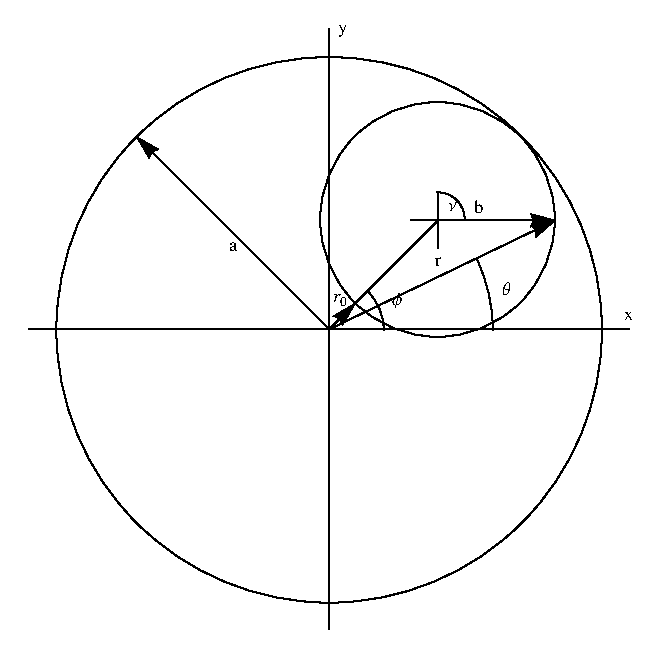
\includegraphics[width=0.9 \textwidth]{dib.eps}
\caption{Contrucci\'on de una hipocicloide: Sea $a$ el radio del circulo mayor y $b$ el radio del circulo menor. Sea $\theta$ el \'angulo que forma el vector de posici\'on del punto sobre el circulo menor con el eje $x$, sea $\phi$ el \'angulo que forma el centro del circulo menor y el eje $x$, finalmente sea $\nu$ el \'angulo que rota el circulo menor sobre un eje fijo. De la condici\'on de no deslizamiento se obtiene que $\nu=\frac{a-b}{b} \phi$. Podemos escribir la posici\'on del punto en t\'erminos de $\phi$ y $\nu$ asi (definimos a $r_0=a-2b$, la distancia mas cercana al centro):
$x=(a-b)\cos \phi-b \cos \nu=\frac{1}{2}\left((a+r_0) \cos (\phi)+(r_0-a) \cos \left(\frac{(a+r_0) \phi}{a-r_0}\right)\right)$
$y=(a-b)\sin \phi+b \sin \nu=\frac{1}{2}\left((a+r_0) \sin (\phi)+(a-r_0) \sin \left(\frac{(a+r_0) \phi}{a-r_0} \right)\right)$}
\label{a}
\end{figure}





Las ecuaciones par\'ametricas de una hipocicloide son:
$$x(\phi)=\frac{1}{2}\left((a+r_{0}) \cos (\phi)+(r_{0}-a) \cos \left(\frac{(a+r_{0}) \phi}{a-r_{0}}\right)\right) $$
$$y(\phi)=\frac{1}{2}\left((a+r_{0}) \sin (\phi)+(a-r_{0}) \sin \left(\frac{(a+r_{0}) \phi}{a-r_{0}}\right)\right) $$
De estas se puede obtener $r(\phi)^2$ asi:
$$r(\phi)^2=x(\phi)^2+y(\phi)^2=$$
$$=\frac{1}{4} \left((a+r_0) \cos (\phi
   )+(r_{0}-a) \cos \left(\frac{(a+r_{0}) \phi
   }{a-r_{0}}\right)\right)^2+\frac{1}{4}
   \left((a+r_{0}) \sin (\phi )+(a-r_{0}) \sin
   \left(\frac{(a+r_{0}) \phi
   }{a-r_{0}}\right)\right)^2$$
Que al simplificar teniendo en cuenta que $\cos^2 x+\sin^2 x=1$, $\cos(a+b)=\cos a \cos b-\sin a \sin b$ y que $(a+b)^2+(a-b)^2=2(a^2+b^2)$ queda:
$$r(\phi)^2=\frac{1}{2}
   \left(a^2+r_{0}^2+\left(r_{0}^2-a^2\right)
   \cos \left(\frac{2 a \phi
   }{a-r_{0}}\right)\right)$$
Por otro lado tambien podemos calcular $\theta(\phi)$:
$$\tan(\theta(\phi))=\frac{y(\phi)}{x(\phi)}=\frac{(a+r_{0}) \sin (\phi )+(a-r_{0}) \sin
   \left(\frac{(a+r_{0}) \phi
   }{a-r_{0}}\right)}{(a+r_{0}) \cos (\phi
   )+(r_{0}-a) \cos \left(\frac{(a+r_{0}) \phi
   }{a-r_{0}}\right)}$$
$$=\frac{a \sin (\phi )+r_{0} \sin (\phi )+a \sin
   \left(\frac{(a+r_{0}) \phi
   }{a-r_{0}}\right)-r_{0} \sin
   \left(\frac{(a+r_{0}) \phi
   }{a-r_{0}}\right)}{a \cos (\phi )+r_{0} \cos
   (\phi )-a \cos \left(\frac{(a+r_{0}) \phi
   }{a-r_{0}}\right)+r_{0} \cos
   \left(\frac{(a+r_{0}) \phi }{a-r_{0}}\right)}$$
$$=\frac{r_{0} \left(\sin (\phi )-\sin
   \left(\frac{(a+r_{0}) \phi
   }{a-r_{0}}\right)\right)+a \left(\sin (\phi
   )+\sin \left(\frac{(a+r_{0}) \phi
   }{a-r_{0}}\right)\right)}{a \left(\cos (\phi
   )-\cos \left(\frac{(a+r_{0}) \phi
   }{a-r_{0}}\right)\right)+r_{0} \left(\cos
   (\phi )+\cos \left(\frac{(a+r_{0}) \phi
   }{a-r_{0}}\right)\right)}$$
Pero recordando las identidades de suma a producto de funciones trigonometricas se tiene:
$$=\frac{2 r_{0} \cos \left(\frac{(a+r_{0}) \phi
   }{2 (a-r_{0})}+\frac{\phi }{2}\right) \sin
   \left(\frac{\phi }{2}-\frac{(a+r_{0}) \phi }{2
   (a-r_{0})}\right)+2 a \cos \left(\frac{\phi
   }{2}-\frac{(a+r_{0}) \phi }{2
   (a-r_{0})}\right) \sin \left(\frac{(a+r_{0})
   \phi }{2 (a-r_{0})}+\frac{\phi }{2}\right)}{2
   r_{0} \cos \left(\frac{\phi
   }{2}-\frac{(a+r_{0}) \phi }{2
   (a-r_{0})}\right) \cos \left(\frac{(a+r_{0})
   \phi }{2 (a-r_{0})}+\frac{\phi }{2}\right)-2 a
   \sin \left(\frac{\phi }{2}-\frac{(a+r_{0}) \phi
   }{2 (a-r_{0})}\right) \sin
   \left(\frac{(a+r_{0}) \phi }{2
   (a-r_{0})}+\frac{\phi }{2}\right)}$$
$$=\frac{a \cos \left(\frac{r_{0} \phi
   }{a-r_{0}}\right) \sin \left(\frac{a \phi
   }{a-r_{0}}\right)-r_{0} \cos \left(\frac{a
   \phi }{a-r_{0}}\right) \sin \left(\frac{r_{0}
   \phi }{a-r_{0}}\right)}{r_{0} \cos
   \left(\frac{a \phi }{a-r_{0}}\right) \cos
   \left(\frac{r_{0} \phi }{a-r_{0}}\right)+a
   \sin \left(\frac{a \phi }{a-r_{0}}\right) \sin
   \left(\frac{r_{0} \phi }{a-r_{0}}\right)}$$
si la anterior ecuaci\'on se divide arriba y abajo por $\cos \left(\frac{a \phi }{a-r_{0}}\right) \cos \left(\frac{r_{0} \phi }{a-r_{0}}\right)$ obtenemos:

$$\tan \theta(\phi)=\frac{a \tan \left ( \frac{a \phi}{a-r_0}\right)-r_0\tan \left ( \frac{r_0 \phi}{a-r_0}\right)}{r_0+a \tan \left ( \frac{a \phi}{a-r_0}\right) \tan \left ( \frac{r_0\phi}{a-r_0}\right)}$$
Note que la \'ultia ecuaci\'on tiene un notable parecido con la identidad para suma de la tangente.\\
Con lo anterior calculado es directo calcular la siguiente cantidad:
$$\tan\left(\theta + \frac{r_0 \phi}{a-r_0}  \right)=\frac{\tan\left( \theta \right)+\tan\left( \frac{r_0 \phi}{a-r_0} \right)}{1-\tan\left( \frac{r_0 \phi}{a-r_0} \right)\tan\left(\theta  \right)}$$
$$=\frac{\frac{a \tan\left( \frac{a \phi}{a-r_0}  \right)-r_0\tan\left( \frac{r_0 \phi}{a-r_0}  \right)+r_0\tan\left( \frac{r_0 \phi}{a-r_0} \right)+a \tan\left( \frac{r_0 \phi}{a-r_0} \right)\tan\left( \frac{a \phi}{a-r_0}  \right)\tan\left( \frac{r_0 \phi}{a-r_0} \right)}{r_0+a \tan \left ( \frac{a \phi}{a-r_0}\right) \tan \left ( \frac{r_0\phi}{a-r_0}\right)}}{\frac{r_0+a \tan\left( \frac{a \phi}{a-r_0} \right) \tan\left( \frac{r_0 \phi}{a-r_0} \right)-\left(a \tan\left( \frac{a \phi}{a-r_0} \right)    -r_0 \tan\left( \frac{r_0 \phi}{a-r_0} \right)\right) \tan\left( \frac{r_0 \phi}{a-r_0} \right)}{r_0+a \tan \left ( \frac{a \phi}{a-r_0}\right) \tan \left ( \frac{r_0\phi}{a-r_0}\right)}}
$$
$$=\frac{a \tan\left( \frac{a \phi}{a-r_0} \right) \left( 1- \tan^2\left( \frac{r_0 \phi}{a-r_0} \right)\right)}{r_0 \left( 1- \tan^2\left( \frac{r_0 \phi}{a-r_0} \right) \right)}$$
Finalmente entonces:
$$\tan\left(\theta + \frac{r_0 \phi}{a-r_0}  \right)=\frac{a \tan\left( \frac{a \phi}{a-r_0} \right)}{r_0}$$
asi $\theta(\phi)$ es:
$$ \theta(\phi)=\tan^{-1}\left(\frac{a}{r_0} \tan\left(\frac{a \phi}{a-r_0} \right) \right)-\frac{r_0 \phi}{a-r_0}$$

Ahora que conocemos $r(\phi)$ y $\theta(\phi)$ podemos calcular $r'(\theta)^2$ asi:
$$\left(\frac{dr}{d\theta}\right)^2=\left(\frac{\frac{dr}{d\phi}}{\frac{d\theta}{d\phi}}\right)^2=
\left(\frac{-\frac{a \left(r_0^2-a^2\right) \sin \left(\frac{2 a \phi }{a-r_0}\right)}{\sqrt{2}
   (a-r_0) \sqrt{a^2+r_0^2+\left(r_0^2-a^2\right) \cos \left(\frac{2 a \phi
   }{a-r_0}\right)}}}{\frac{a^2 \sec ^2\left(\frac{a \phi }{a-r_0}\right)}{(a-r_0) r_0
   \left(\frac{a^2 \tan ^2\left(\frac{a \phi
   }{a-r_0}\right)}{r_0^2}+1\right)}-\frac{r_0}{a-r_0}}\right)^2
=-\frac{a^2 \left(-a^2-r_0^2+\left(a^2-r_0^2\right) \cos \left(\frac{2 a \phi
   }{a-r_0}\right)\right) \tan ^2\left(\frac{a \phi }{a-r_0}\right)}{2 r_0^2}
$$



Por otro lado si calculamos el lado izquierdo de la ecuaci\'on diferencial 
$$\frac{a^2 r^2}{a^2-r^2}\frac{r^2-r_0^2}{r_0^2}=\frac{a^2 \left(a^2+r_0^2+\left(r_0^2-a^2\right) \cos \left(\frac{2 a \phi
   }{a-r_0}\right)\right) \left(\frac{1}{2}
   \left(a^2+r_0^2+\left(r_0^2-a^2\right) \cos \left(\frac{2 a \phi
   }{a-r_0}\right)\right)-r_0^2\right)}{2 r_0^2 \left(a^2+\frac{1}{2}
   \left(-a^2-r_0^2-\left(r_0^2-a^2\right) \cos \left(\frac{2 a \phi
   }{a-r_0}\right)\right)\right)}$$ 


Que al simplificar se convierte en:
$$-\frac{a^2 \left(-a^2-r_{0}^2+(a-r_{0})
   (a+r_{0}) \cos \left(\frac{2 a \phi
   }{a-r_{0}}\right)\right) \tan ^2\left(\frac{a
   \phi }{a-r_{0}}\right)}{2 r_{0}^2}$$
Lo que muestra que efectivamente hemos encontrado la soluci\'on al problema.
\\
Por \'ultimo queremos calcular el tiempo de viaje y la profundidad m\'axima alcanzada en funci\'on de la separaci\'on angular de los puntos sobre la tierra.
Para encontrar las anteriores cantidades primero notemos $r_0\leq r\leq a$ y que $r_0=r \rightarrow \phi=0 \rightarrow \theta=0$, es decir por la forma como construimos la soluci\'on $r$ es m\'inimo en $\theta=0$. Ahora podemos buscar $\theta$ tal que $r=a$, para ello primero encontremos  a $\phi$ que cumpla esa condici\'on:

$$a^2=\frac{1}{2}
   \left(a^2+r_{0}^2+\left(r_{0}^2-a^2\right)
   \cos \left(\frac{2 a \phi
   }{a-r_{0}}\right)\right) \rightarrow \phi=\frac{\pi}{2} \frac{a-r_0}{a}
$$
Si reemplazamos lo anterior en la ecuaci\'on para $\theta$ se obtiene que:
$$\theta(r=a)=\frac{\pi}{2}\left(1-\frac{r_0}{a}\right)$$
Asi entonces el anterior es el \'angulo se barre entre ir de la superficie al punto de maximo acercamiento, por razones de simetr\'ia este debe ser igual al \'angulo que se barre en ir desde el punto de m\'aximo acercamiento al centro hasta la superficie de nuevo. De lo anterior se deduce entonces que si en el trayecto de viaje de el vehiculo se acerca hasta el centro $r_0$ entonces los puntos estan separados angularmente una distancia $\alpha=\pi \left(1-\frac{r_0}{a}\right)$. Como es de esperarse si los dos puntos son diametramente opuestos entonces $r_0=0$ y la trayectoria pasa por el centro y ademas como se comprueba facilmente es una linea recta en la que se presenta movimiento arm\'onico simple.\\
Finalmente la integral que da el tiempo de viaje se puede reparametrizar en terminos de $\phi$ para obtener:
$$
t_{min}=\sqrt{\frac{m}{k}}\int_{-\frac{\pi}{2}(1-\frac{r_0}{a})}^{\frac{\pi}{2}(1-\frac{r_0}{a})} 
\sqrt{\frac{\left(\frac{dr}{d\phi} \right)^2+r^2(\phi)\left(\frac{d\theta}{d\phi} \right)^2}{a^2-r^2(\phi)}} d\phi=\sqrt{\frac{m}{k}} \frac{\pi}{a}\sqrt{a^2-r_0^2}=\sqrt{\frac{m}{k}} \pi\sqrt{1-\left(\frac{r_0}{a}\right)^2}
$$

Pero $\frac{r_0}{a}=1-\frac{\alpha}{\pi}$ as\'i que el tiempo m\'inimo en t\'erminos de la separaci\'on angular es:
$$
t_{min}=\sqrt{\frac{m}{k}} \pi \sqrt{1-\left(1-\frac{\alpha}{\pi}\right)^2}
$$
Finalmente se pide hallar el tiempo de viaje entre Los \'Angeles y Nueva York, estos estan separados una distancia de $4800 km$, ademas se sabe que el diametro de la Tierra es de aproximadamente $a=6400 km$ luego su separaci\'on angular es de $\alpha=\frac{4800}{6400}=0.75$ ademas la masa de la Tierra es de $M=6.0\cdot10^{24} kg$ y la constante de Cavendish tiene un valor de $G=6.7 \cdot 10^{-11} m^3 kg^{-1} s^{-2}$ entonces $\frac{k}{m}=1.5 \cdot 10^{-6} s^{-2}$.\\
El tiempo de viaje de Nueva York a Los \'Angeles es $t_{NY-LA}=1.64\cdot10^3 s=27'$ y el radio m\'inimo es $r_0=a \left(1-\frac{0.75}{\pi}\right)=4.9\cdot 10^3 km$.









\section*{Ejercicio 2.16}
Para el presente problema el Lagrangiano est\'a dado por :
\begin{equation}
e^{t \gamma } \left(\frac{1}{2} m
   \dot q(t)^2-\frac{1}{2} k q(t)^2\right)
\label{kl}
\end{equation}
La ecuaci\'on de Euler Lagrange para el anterior Lagrangiano es:
\begin{equation}
e^{t \gamma } \left(k q(t)+m \left(\gamma 
   \dot q(t)+\ddot q(t)\right)\right)=0
\end{equation}
Que es la ecuaci\'on de movimiento de un oscilador arm\'onico amortiguado.
Si se hace la transformaci\'on de coordenadas $q=e^{-\frac{t \gamma }{2}} s $ el Lagrangiano toma la forma siguiente:
\begin{equation}
\frac{1}{8} \left(\left(m \gamma ^2-4 k\right)
   s(t)^2-4 m \gamma  \dot s(t) s(t)+4 m
   \dot s(t)^2\right)
\end{equation}
La ecuaci\'on de Euler lagrange es:
\begin{equation}
\left(m \gamma ^2-4 k\right) s(t)=4 m \ddot s(t)
\end{equation}
Esta es la ecuaci\'on de movimiento de un oscilador arm\'onico.
Finalmente la funci\'on $h$ de Jacobi para el anterior Lagrangiano es constante de movimiento, si se expresa en t\'erminos de $q(t)$ queda ($\omega^2=k/m$):
\begin{equation}
 \frac{1}{2} e^{t \gamma } \left(\omega ^2
   q(t)^2+\gamma  \dot q(t) q(t)+\dot q(t)^2\right)
\end{equation}
Que es la constante de movimiento para el oscilador arm\'onico amortiguado.
 


\section*{Ejercicio 2.18}
Para este caso usando coordenadas esf\'ericas tenemos lo siguiente:
\begin{eqnarray}
T=\frac{1}{2} a^2 m \left(\theta '^2+\sin ^2(\theta
   ) \phi '^2\right)\\
V=mgz=m g a \cos (\theta )
\end{eqnarray}
Pero $\phi=\omega t$. As\'i el lagrangiano es:
\begin{equation}
L=T-V=\frac{1}{2} a^2 m \left(\theta '^2+\sin ^2(\theta
   ) (\omega)^2\right)-m g a \cos (\theta )
\end{equation}
La ecuaci\'on de Euler-Lagrange que satisface $\theta$ es:
\begin{equation}
a m \left(\left(a \cos (\theta ) \omega ^2+g\right)
   \sin (\theta )-a \theta ''\right)=0
\label{el}
\end{equation}
Como se ve de el lagrangiano la cantidad  $h$ (la funci\'on de energia) es conservada ya que el lagrangiano no depende explicitamente del tiempo. Como adem\'as contiene  $\theta$ el momento generalizado $p_\theta=a^2 m \theta '$ no se conserva.
Para hallar condiciones de equilibrio hagamos $\theta'=0\Longrightarrow \theta''=0$. Esto implica en (\ref{el}) que:
\begin{equation}
 \left(a \cos (\theta ) \omega ^2+g\right) \sin
   (\theta )=0
\label{iii}
\end{equation}
La anterior ecuaci\'on implica o bien que $\theta=0$ o $\theta=\pi$ o que $\omega=\sqrt{\frac{-g}{a \cos(\theta)}}$. El m\'inimo valor que toma $\omega$ es $\omega_0=\sqrt{\frac{g}{a}}$. Para valores de $\omega$ menores que $\omega_0$ la ecuaci\'on (\ref{iii}) no tiene soluciones reales excepto las triviales(0 y $\pi$), es decir no hay mas puntos de equilibrio.

\section*{Ejercicio 2.24}
\begin{eqnarray}
\label{ecu}
 x&=&\sum_{j=0}^\infty a_j \cos(j \omega t)\\
\dot x&=&-\sum_{j=0}^\infty a_j \omega j \sin(j \omega t)\\
L&=&\frac{m \dot x^2}{2}-\frac{k x^2}{2}\\
S&=&\int_{0}^{\frac{2 \pi}{\omega}} L dt
\end{eqnarray}
Si sustitimos $x$ y $\dot x$ en $L$ obtenemos:
\begin{eqnarray}
L=\frac{m (-\sum_{j=0}^\infty a_j \omega j \sin(j \omega t))^2}{2}-\frac{k (\sum_{j=0}^\infty a_j \cos(j \omega t))^2}{2}\\
L=\frac{m( \sum_{j=0}^\infty a_j^2 \omega^2 j^2 \sin^2(j \omega t)- 2\sum_{i=0}^{\infty}\sum_{i<j}^\infty a_j a_i \omega^2 i j \sin(j \omega t) \sin(i \omega t) )}{2}-\\
\frac{k( \sum_{j=0}^\infty a_j^2 \cos^2(j \omega t)+ 2\sum_{i=0}^{\infty}\sum_{i<j}^\infty a_j a_i \cos(j \omega t) \sin(i \omega t) )}{2}
\end{eqnarray}
Al hacer la integral los t\'erminos cruzados con diferente \'indice se anulan i.e. si  $i\neq j$:
\begin{equation}
\int_{0}^{\frac{2 \pi}{\omega}} \sin(i \omega t) \sin(j \omega t) dt=\int_{0}^{\frac{2 \pi}{\omega}} \cos(i \omega t) \cos(j \omega t) dt=0 
\end{equation}
Por otro lado las integrales con t\'erminos no cruzados son facilmente calculadas as\'i:
\begin{eqnarray}
 \int_{0}^{\frac{2 \pi}{\omega}} \cos^2(0)dt=\frac{2 \pi}{\omega}\\
\int_{0}^{\frac{2 \pi}{\omega}} \sin^2(0)dt=0\\
\int_{0}^{\frac{2 \pi}{\omega}} \cos^2(j \omega t)dt=\frac{\pi}{\omega}\\
\int_{0}^{\frac{2 \pi}{\omega}} \sin^2(j \omega t)dt=\frac{\pi}{\omega}
\end{eqnarray}
La acci\'on $S$ toma la siguiente forma:
\begin{eqnarray}
 S=\frac{m\sum_{j=1}^\infty a_j^2 \omega^2 j^2 \frac{\pi}{\omega}}{2}-\frac{k( \frac{2\pi}{\omega}a_0^2+\sum_{j=1}^\infty a_j^2 \frac{\pi}{\omega})}{2}\\
S=-\frac{k\pi}{\omega}a_0^2+\frac{\pi}{2} \sum_{j=1}^\infty a_j^2(m \omega j^2-\frac{k}{\omega})
\end{eqnarray}
La acci\'on es ahora una funci\'on de las $a_j$, por lo tanto para que sea extremo el gradiente $\nabla_a$ de la acci\'on con respecto a las $a_j$ debe ser $0$, es decir el vector infinito con entradas:
\begin{equation}
\left( \frac{-2 k \pi a_0}{\omega},...,\pi a_j (m j^2 \omega-\frac{k}{ \omega}),... \right)
\end{equation}
Debe ser el vector nulo. Claramente lo anterior implica que $a_0=0$ y que todos los $a_j$ excepto uno deben ser 0. El que no es cero debe ser tal que $\pi a_i (m i^2 \omega-\frac{k}{ \omega})=0$ es decir $\omega=\frac{1}{i}\sqrt{\frac{k}{m}}$. Si reemplazamos en (\ref{ecu}) obtenemos que 
\begin{equation}
x=a_i \cos(i \frac{1}{i}\sqrt{\frac{k}{m}} t)=a_i \cos(\sqrt{\frac{k}{m}} t)= \sum_{j=0}^\infty a_j \cos(j \omega t)
\label{casi}
\end{equation}
Pero por hip\'otesis el periodo de $x$ es $\frac{2\pi}{\omega}$ y por otro lado el periodo de la funci\'on de la ecuaci\'on (\ref{casi}) es $\frac{2\pi}{\sqrt{\frac{k}{m}}}$, entonces $\omega^2=\frac{k}{m}$ y $a_i$=$a_1$.

\end{document}

\section*{Cap\'itulo 8}
\documentclass[letterpaper,10pt]{article}
\usepackage[latin1]{inputenc}
\usepackage[dvips]{graphicx}
\usepackage[spanish]{babel}


\textwidth = 16.5 cm
\textheight = 23.5 cm
\oddsidemargin = 0.0 cm
\evensidemargin = 0.0 cm
\topmargin = 0.0 cm
\headheight = 0.0 cm
\headsep = 0.0 cm 

%opening
\title{Ejercicios del cap\'itulo 8 de\\ \emph{Classical Mechanics} de H. Goldstein}
\author{Nicol\'as Quesada M. \\ {\small \sf Instituto de F\'isica, Universidad de Antioquia}}
\date{}

\begin{document}

\maketitle

\section*{Ejercicio 8.2}
Supongamos que tenemos un Lagrangiano $L(q_i,\dot q_i,t)$, con su respectivo Hamiltoniano $H$, y momentos conjugados $p_i$. Se desea averiguar como queda el nuevo Hamiltoniano $H'$ y los nuevos momentos conjugados $p_i'$ si se usa un nuevo Lagrangiano $L'=L+\frac{dF}{dt}$ donde $F$ es una funci\'on arbitraria pero diferenciable.
Los nuevos momentos generalizados vienen dados por:
$$
p'_i=\frac{\partial L'(q_i,\dot q_i,t)}{\partial \dot q_i}=\frac{\partial L}{\partial \dot q_i}+\frac{\partial \left(\frac{dF}{dt} \right)}{\partial \dot q_i}
$$
Pero el \'ultimo t\'ermino puede transformarse asi: (Suma sobre \'indices repetidos):
$$
\frac{\partial \left(\frac{dF}{dt} \right)}{\partial \dot q_i}=\frac{\partial \left( \frac{\partial F}{\partial q_j} \dot q_j+\frac{\partial F}{\partial t} \right)}{\partial \dot q_i}=\frac{\partial F}{\partial q_i}
$$
Teniendo en cuanto lo anterior y que $p_i=\frac{\partial L(q_i,\dot q_i,t)}{\partial \dot q_i}$ tenemos que:
$$
p'_i=p_i+\frac{\partial F}{\partial q_i}
$$
El nuevo Hamiltoniano est\'a dado por: 
$$
H'=\dot q_i p'_i-L'=\dot q_i (p_i+\frac{\partial F}{\partial q_i})-L-\frac{dF}{dt}=\dot q_i (p_i+\frac{\partial F}{\partial q_i})-L-(\frac{\partial F}{\partial q_i} \dot q_i+\frac{\partial F}{\partial t})$$ $$
H'=\dot q_i p_i-L-\frac{\partial F}{\partial t}=H-\frac{\partial F}{\partial t}
$$
Para mostrar que las ecuaciones que se obtienen con este nuevo Hamiltoniano para $p_i'$ y $q_i$ tienen la misma forma que las que se obtienen para $p_i$ y $q_i$ atrav\'es del Hamiltoniano original escribamos el principio de Hamilton para el antiguo Hamiltoniano $H$ teniendo en cuenta la adici\'on de $\frac{dF}{dt}$:\\
$$\delta I=\delta \int_{t_1}^{t_2} L+\frac{dF}{dt}dt=\delta \int_{t_1}^{t_2}(p_i \dot q_i-H+\frac{dF}{dt})dt=\delta \int_{t_1}^{t_2}(p_i \dot q_i-H+\frac{\partial F}{\partial q_i} \dot q_i+\frac{\partial F}{\partial t})dt$$
Los t\'erminos dentro de la integral se pueden reorganizar para obtener:
$$ \delta \int_{t_1}^{t_2}((p_i+\frac{\partial F}{\partial q_i} )\dot q_i-(H- \frac{\partial F}{\partial t}))dt$$
Pero el primer par\'entesis resulta ser $p_i'$ y el segundo $H'$ asi:
$$ \delta \int_{t_1}^{t_2}(p_i'\dot q_i-H')dt$$
En este punto podemos asumir que $H'$ esta escrito en t\'erminos de las $q_i$ y las nuevas $p_i'$ y asi podemos usar las ecuaciones de Euler-Lagrange para hallar:
$$
\frac{d}{dt}\left( \frac{\partial f}{\partial \dot q_i}\right)-\frac{\partial f}{\partial q_i}=\dot p_i'+\frac{\partial H'}{\partial q_i}=0$$ 
$$
\frac{d}{dt}\left( \frac{\partial f}{\partial \dot p_i'}\right)-\frac{\partial f}{\partial p_i'}=\dot q_i-\frac{\partial H'}{\partial p_i'}=0
$$
Que son las ecuaciones de Hamilton para las variables $(q_i,p_i')$\\
\\

Para el resto de ejercicios $a'$ denota la derivada total de la variable $a$ con respecto al tiempo $t$.\\


\section*{Ejercicio 8.9}
Para este problema se hace un procedimiento an\'alogo al que se hace en la formulaci\'on lagrangiana. Asi entonces:
$$
\delta S=\delta \int_{t_1}^{t_2} q_i' p_i-H(q_j,p_j,t)-\lambda_i \psi_i(q_j,p_j,t)dt
$$
La variaci\'on se puede hacer  ahora con $n$ $\delta q_i$, $n$ $\delta p_i$ y $m$ $\lambda_i$.
Para esta problema las $2n$ ecuaciones de Euler-Lagrange de interes son (siendo $f$ el integrando de la ecuaci\'on anterior y $k=1,...,n$):
$$
\frac{d}{dt}\left( \frac{\partial f}{\partial q_k'}\right)-\frac{\partial f}{\partial q_k}=0$$ $$
\frac{d}{dt}\left( \frac{\partial f}{\partial p_k'}\right)-\frac{\partial f}{\partial p_k}=0
$$
Sustituyendo para las primeras $n$ ecuaciones obtenemos:
$$
\frac{d}{dt}\left( \frac{\partial (q_i' p_i-H(q_j,p_j,t)-\lambda_i \psi_i(q_j,p_j,t))}{\partial q_k'}\right)-\frac{\partial (q_i' p_i-H(q_j,p_j,t)-\lambda_i \psi_i(q_j,p_j,t))}{\partial q_k}=0$$ $$
\frac{d p_k}{dt}-(\frac{\partial (-H(q_j,p_j,t)-\lambda_i \psi_i(q_j,p_j,t))}{\partial q_k})=0
$$
Reorganizando t\'erminos  y teniendo en cuenta que hay suma sobre el \'indice repetido $i$ nos queda:
$$
-p'_k=\frac{\partial H}{\partial q_k}+\lambda_i \frac{\partial \psi_i(q_j,p_j,t)}{\partial q_k}
$$
Para las restantes $n$ ecuaciones tenemos:
$$
\frac{d}{dt}\left( \frac{\partial (q_i' p_i-H(q_j,p_j,t)-\lambda_i \psi_i(q_j,p_j,t))}{\partial p_k'}\right)-\frac{\partial (q_i' p_i-H(q_j,p_j,t)-\lambda_i \psi_i(q_j,p_j,t))}{\partial p_k}=0
$$
Reorganizando los t\'erminos tenemos (De nuevo suma sobre $i$):
$$0-\left(q'_k-\frac{\partial H}{\partial p_k}-\lambda_i \frac{\partial \psi_i(q_j,p_j,t)}{\partial p_k}\right)=0$$ o $$q'_k =\frac{\partial H}{\partial p_k}+\lambda_i \frac{\partial \psi_i(q_j,p_j,t)}{\partial p_k} $$

\section*{Ejercicio 8.12}
Usando la convenci\'on usada en el cap\'itulo 2 el lagrangiano del sistema se puede escribir como:
$$ L=\frac{m_1+m_2}{2} \textbf{r'}^2+\frac{1}{2}\frac{m_1 m_2}{m_1+m_2} \textbf{R'}^2-U(R)$$
Usando coordenadas esfericas $R,\theta,\phi$ para $\textbf{R}$ y coordenadas rectangulares $x,y,z$ para $\textbf{r}$ y llamando $\mu$=$\frac{m_1 m_2}{m_1+m_2}$ y $M=m_1+m_2$ tenemos:

$$ L=\frac{\mu}{2}(R'^2+R^2 \theta'^2+R^2 \sin^2 (\theta) \phi'^2)+\frac{M}{2}(x'^2+y'^2+z'^2)-U(R)$$

De lo anterior se ve facilmente que el Hamiltoniano del sistema es:
$$H=\frac{1}{2\mu}(p_R^2+\frac{ p_\theta^2}{R^2}+\frac{p_\phi^2}{R^2 \sin^2 (\theta)})+\frac{1}{2 M}(p_x^2+p_y^2+p_z^2)+U(R)$$
Ahora obtegamos la ecuaciones de Hamilton para $p_x, p_y ,p_z, x, y ,z$ que son:
$$p_x'=-\frac{\partial H}{\partial x}=0\Rightarrow p_x=c_1$$
$$p_y'=-\frac{\partial H}{\partial y}=0\Rightarrow p_y=c_2$$
$$p_z'=-\frac{\partial H}{\partial z}=0\Rightarrow p_z=c_3$$
$$x'=\frac{\partial H}{\partial p_x}=p_x/M\Rightarrow x=x_0+(p_x/M)t$$
$$y'=\frac{\partial H}{\partial p_y}=p_x/M\Rightarrow y=y_0+(p_y/M)t$$
$$z'=\frac{\partial H}{\partial p_z}=p_x/M\Rightarrow z=z_0+(p_z/M)t$$
Con lo anterior nos hemos librado de la mitad de las variables y podemos escribir el Hamiltoniano de la siguiente manera:
$$ H=\frac{1}{2\mu}(p_R^2+\frac{ p_\theta^2}{R^2}+\frac{p_\phi^2}{R^2 \sin^2 (\theta)})+U(R)+c$$
Donde $c=\frac{1}{2 M}(p_x^2+p_y^2+p_z^2)$. De ahora en adelante dicha constante se omitira ya que no afecta las ecuaciones de movimiento de las dem\'as variables. En el anterior Hamiltoniano la variable $\phi$ es c\'iclica por lo que $p_\phi=l_z$ es constante de movimiento y asi:

$$ H=\frac{1}{2\mu}(p_R^2+\frac{ p_\theta^2}{R^2}+\frac{l_z^2}{R^2 \sin^2 (\theta)})+U(R)= \frac{1}{2\mu}(p_R^2+\frac{1}{R^2}(p_\theta^2+\frac{l_z^2}{\sin^2 (\theta)}))+U(R)=\frac{1}{2\mu}(p_R^2+\frac{f(\theta,p_\theta)}{R^2}))+U(R)$$
Ahora como en ves de $\theta$ y $p_\theta$ por separado aparece una funci\'on  $f(\theta,p_\theta)$ de las dos esta debe ser una constante de movimientom \emph{i.e.} 
$$f(\theta,p_\theta)=L^2=p_\theta^2+\frac{l_z^2}{\sin^2 (\theta)}=k$$
De la anterior ecuaci\'on podemos obtener $p_\theta$ en t\'erminos de $\theta$ asi:
$$p_\theta=\pm \sqrt{L^2-\frac{l_z^2}{\sin^2(\theta)}}$$ y ademas podemos escribir el Hamiltoniano asi:
$$H=\frac{1}{2\mu}(p_r^2+\frac{L^2}{R^2})+U(r) $$
Finalmente podemos obtener $p_R$ en funci\'on de $r$ como ($H=E=$ constante de Movimiento):
$$p_R=\pm \sqrt{2 \mu (H-U(r)-\frac{L^2}{2 R^2})}=\pm \sqrt{2 \mu (E-U(r)-\frac{L^2}{2 R^2})}  $$

Con lo anterior en mente podemos escribir las restantes ecuaciones de Hamilton:
$$p_R'=-\frac{\partial H}{\partial R}=\frac{L^2}{\mu R^3}-\frac{\partial U}{\partial R}\Rightarrow p_R-p_{R_0}=\int_{0}^{t} \frac{L^2}{\mu R^3}-\frac{\partial U}{\partial R} dt$$
$$p_\theta'=-\frac{\partial H}{\partial \theta}=\frac{\cos(\theta)}{\sin^3(\theta)}\frac{l_z^2}{\mu R^2}\Rightarrow p_\theta-p_{\theta_0}=\int_{0}^{t} \frac{\cos(\theta)}{\sin^3(\theta)}\frac{l_z^2}{\mu R^2} dt$$
$$p_\phi'=-\frac{\partial H}{\partial \phi}=0\Rightarrow p_\phi=l_z$$
$$R'=\frac{\partial H}{\partial p_R}=p_r/\mu \Rightarrow t=\int_{R_0}^{R} \frac{dR}{\sqrt{\frac{2 }{\mu}(E-U-\frac{L^2}{2mR^2})}}$$
$$\theta'=\frac{\partial H}{\partial p_\theta}=p_\theta/(R^2 \mu)\Rightarrow \int_0^t \frac{dt}{\mu R^2}=\int_{\theta_0}^{\theta}\frac{d\theta}{\sqrt{L^2-\frac{l_z^2}{\sin^2{\theta}}}}$$
$$\phi'=\frac{\partial H}{\partial p_\phi}=l_z/(\mu R^2 \sin^2(\theta))\Rightarrow \phi-\phi_0=l_z \int_0^t \frac{dt}{m R^2 \sin^2(\theta)}$$
Note que una vez realizada la integral correspodiente a $R'$ y obtenido $R(t)$ en forma explicita este se puede reemplazar en la integral correspodiente a $\theta'$ y asi obtener $\theta$ como funci\'on explicita de $t$. Con estas dos variables conocidas se puede sustituir en la ecuaciones de las dem\'as variables, realizar las respectivas integraciones e inversiones y resolver el problema completamente.




\section*{Ejercicio 8.14}
Sea $L=a x'^2+\frac{b y'}{x}+c x' y'+ f y^2x' z' +g y'-k \sqrt{x^2+y^2}$. De este obtenemos los momentos conjugados:
$$p_x=f z' y^2+2 a x'+c y'$$
$$p_y=\frac{b}{x}+g+c x'$$ 
$$p_z=f y^2 x'$$
Con estos podemos obtener el Hamiltoniano:
$$
H=q_i' p_i-L=(f x' z' y^2+\left(\frac{b}{x}+g+c x'\right) y'+x' \left(f z' y^2+2 a x'+c y'\right))$$ $$-(a x'^2+\frac{b y'}{x}+c x' y'+ f y^2x' z' +g y'-k \sqrt{x^2+y^2})$$ $$
H=(2 f x' z' y^2+2 a x'^2+g y'+2 c x' y'+\frac{b y'}{x})-(a x'^2+\frac{b y'}{x}+c x' y'+ f y^2x' z' +g y'-k \sqrt{x^2+y^2})$$ $$
H=a x'^2+\left(f z' y^2+c y'\right) x'+k \sqrt{x^2+y^2}
$$
Aunque la transformaci\'on (lineal) que manda a las velocidades en los momentos no tiene inversa lo que si se puede hacer es de la ecuaci\'on de $p_x$ despejar $y'$ y de la de $p_z$ a $x'$ para obtener:
$$
y'=\frac{-f z' y^2+p_x-2 a x'}{c}=\frac{-f z' y^2+p_x-2 a \frac{p_z}{f y^2}}{c}$$ $$
x'=\frac{p_z}{f y^2}
$$

y sustituirlos en la ecuaci\'on del Hamiltoniano:
$$
H=a x'^2+\left(f z' y^2+c \frac{-f z' y^2+p_x-2 a x'}{c}\right) x'+k \sqrt{x^2+y^2}$$ $$
H=\frac{a p_z^2}{f^2 y^4}+\frac{\left(p_x-\frac{2 a p_z}{f y^2}\right) p_z}{f y^2}+k \sqrt{x^2+y^2}$$ $$
H=-\frac{a p_z^2}{f^2 y^4}+\frac{p_x p_z}{f y^2}+k \sqrt{x^2+y^2}
$$
Este Hamiltoniano no depende ni de $p_y$ ni de $z$, por lo tanto $y=c$ y $p_z=k$ son constantes de movimiento. Adem\'as $H$ no depende explicitamente de $t$ por lo tanto $H$ tambien es constante de movimiento


\section*{Ejercicio 8.19}
Del dibujo se ve que la posici\'on del cuerpo puede ser escrita asi:
$$
\tilde{x}=l \sin (\theta )+x$$ $$
\tilde{z}=-l \cos (\theta )+z=a x^2-l \cos (\theta )
$$
Donde $\theta$ es el \'angulo que forma el eje del p\'endulo con la vertical. As\'i el lagrangiano toma la siguiente forma:
$$
L=\frac{1}{2} m \left(\tilde{x}'^2+\tilde{z}'^2\right)-m g \tilde{z}
$$
Usando como coordenadas generalizadas $x$ y $\theta $ se reescribe asi:
$$
\frac{1}{2} m \left(\left(x'+l \cos (\theta ) \theta '\right)^2+\left(2 a x x'+l
   \sin (\theta ) \theta '\right)^2\right)- m g \left(a x^2-l \cos (\theta )\right)
$$
Expandiendo:
$$
L=2 a^2 m x'^2 x^2-a g m x^2+2 a l m \sin (\theta ) x' \theta ' x+\frac{1}{2}
   m x'^2+\\ \frac{1}{2} l^2 m \cos ^2(\theta ) \theta '^2+\frac{1}{2} l^2 m \sin ^2(\theta
   ) \theta '^2+g l m \cos (\theta )+l m \cos (\theta ) x' \theta '
$$
Lo que puede ser reescrito asi:
$$
L=L_0+\frac{1}{2} \textbf{q'}^T T \textbf{q'}
$$
con:
$$
\textbf{q'}=\left(
\begin{array}{l}%[pos]{spalten}
x'\\
\theta'
\end{array} \right)$$ $$
T=
\left(
\begin{array}{ll}
 4 a^2 m x^2+m & l m \cos (\theta )+2 a l m \sin (\theta ) x \\
 l m \cos (\theta )+2 a l m \sin (\theta ) x & l^2 m
\end{array}
\right)$$ $$
L_0=g l m \cos (\theta )-a g m x^2 $$

Para hallar el Hamiltoniano se usa el procedimiento  de la ecuaci\'on 8.27 p\'agina 340 cap\'itulo 8:
$$
H(q,p,t)=\frac{1}{2} \textbf{p}^T T^{-1} \textbf{p}-L_0(q,t)
$$
Para este caso la inversa de $T$ es:
$$
T^{-1}=\frac{1}{\det(T)} \left(
\begin{array}{ll}
 l^2 m & -2 a l m \sin (\theta ) x-l m \cos (\theta ) \\
 -2 a l m \sin (\theta ) x-l m \cos (\theta ) & 4 a^2 m x^2+m
\end{array}
\right)$$ $$
\det(T)=l^2 m^2-l^2 \cos ^2(\theta ) m^2+4 a^2 l^2 x^2 m^2-4 a^2 l^2 \sin ^2(\theta ) x^2
   m^2-4 a l^2 \cos (\theta ) \sin (\theta ) x m^2 $$ $$
\det(T)=m^2 l^2 (\sin(\theta)^2+4 a^2 x^2 \cos^2(\theta)-4 a x \cos (\theta ) \sin (\theta ) )$$ $$
\det(T)=m^2 l^2 (\sin(\theta)-2 a x \cos(\theta))^2
$$

$$
\frac{\textbf{p}^T T^{-1} \textbf{p}}{2}=\frac{1}{2 \det(T)} \left(p_x {} p_\theta \right) \left(
\begin{array}{ll}
 l^2 m & -l m \cos (\theta )-2 a l m \sin (\theta ) x \\
 -l m \cos (\theta )-2 a l m \sin (\theta ) x & 4 a^2 m x^2+m
\end{array}
\right) \left(
\begin{array}{l}
 p_x \\
 p_{\theta }
\end{array}
\right)$$ $$
\frac{\textbf{p}^T T^{-1} \textbf{p}}{2}=\frac{m \left(l^2 p_x^2-2 l p_{\theta } p_x (\cos (\theta )+2 a \sin (\theta ) x)+p_{\theta }^2 \left(4 a^2 x^2+1\right)\right)}{2 \det (T)}
$$
Finalmente el Hamiltoniano queda asi:
$$
H=\frac{m \left(l^2 p_x^2-2 l p_{\theta } p_x (\cos (\theta )+2 a \sin (\theta ) x)+p_{\theta }^2 \left(4 a^2 x^2+1\right)\right)}{2 \det (T)}-m g l \cos (\theta )+m a g x^2$$ $$
H=\frac{l^2 p_x^2-2 l p_{\theta } p_x (\cos (\theta )+2 a \sin (\theta ) x) +p_{\theta }^2 \left(4 a^2 x^2+1\right)}{2 l^2 m (\sin (\theta )-2 a \cos (\theta ) x)^2}-m g l\cos (\theta )+ m g a x^2
$$
Ahora con el hamiltoniano hallamos las ecuaciones de Hamilton:

$$x'=\frac{\partial H}{\partial p_x}=\frac{l p_x-(\cos (\theta )+2 a \sin (\theta ) x) p_{\theta }}{l m (\sin (\theta)-2 a \cos (\theta ) x)^2}$$

$$\theta'=\frac{\partial H}{\partial p_\theta}=\frac{\left(4 a^2 x^2+1\right) p_{\theta }-l (\cos (\theta )+2 a \sin (\theta ) x) p_x}{l^2 m (\sin (\theta )-2 a \cos (\theta ) x)^2}$$

$$p_x'=-\frac{\partial H}{\partial x}=\frac{2 a}{m} \left( -g x m^2+\frac{p_{\theta } \left(l \sin (\theta ) p_x-2 a x p_{\theta   }\right)}{l^2 (\sin \theta -2 a x \cos \theta )^2}  -\frac{\cos (\theta ) \left(l^2 p_x^2-2 l (\cos (\theta )+2 a \sin (\theta ) x) p_{\theta }  p_x+\left(4 a^2 x^2+1\right) p_{\theta }^2\right)} {l^2 (\sin (\theta )-2 a \cos (\theta ) x)^3} \right) $$

\begin{eqnarray*}
p_\theta'&=&-\frac{\partial H}{\partial \theta}= \frac{1}{l^2 m} \left(-g m^2 \sin (\theta ) l^3+\frac{p_x p_{\theta } l}{2 a \cos (\theta ) x-\sin(\theta )} \right)\\
& &+\frac{1}{l^2 m} \left(\frac{(\cos (\theta )+2 a \sin (\theta ) x) \left(l^2 p_x^2-2 l(\cos (\theta )+2 a \sin (\theta ) x) p_{\theta } p_x+\left(4 a^2 x^2+1\right) p_{\theta }^2\right)}{(\sin (\theta )-2 a \cos (\theta ) x)^3} \right)
\end{eqnarray*}

La anteriores expresi\'ones para $p_x'$ y $p_\theta'$ se pueden reorganizar asi:
$$
p_\theta'=\frac{(\cos (\theta )+2 a \sin (\theta ) x) p_x^2}{m (\sin (\theta )-2 a \cos(\theta ) x)^3}$$ $$+\left(\frac{2 a \cos (\theta ) x-\sin (\theta )}{l m (\sin(\theta )-2 a \cos (\theta ) x)^2}-\frac{2 (\cos (\theta )+2 a \sin (\theta )x)^2}{l m (\sin (\theta )-2 a \cos (\theta ) x)^3}\right) p_{\theta }p_x$$ $$+\frac{(\cos (\theta )+2 a \sin (\theta ) x) \left(4 a^2 x^2+1\right)p_{\theta }^2}{l^2 m (\sin (\theta )-2 a \cos (\theta ) x)^3}-g l m \sin (\theta)
$$
$$
p_x'=-\frac{2 a \cos (\theta ) p_x^2}{m (\sin (\theta )-2 a \cos (\theta )
   x)^3}$$ $$+\left(\frac{2 a \sin (\theta )}{l m (\sin (\theta )-2 a \cos (\theta )
   x)^2}+\frac{4 a \cos (\theta ) (\cos (\theta )+2 a \sin (\theta ) x)}{l m (\sin
   (\theta )-2 a \cos (\theta ) x)^3}\right) p_{\theta } p_x+$$ $$\left(-\frac{4 x
   a^2}{l^2 m (\sin (\theta )-2 a \cos (\theta ) x)^2}-\frac{2 \cos (\theta ) \left(4
   a^2 x^2+1\right) a}{l^2 m (\sin (\theta )-2 a \cos (\theta ) x)^3}\right)
   p_{\theta }^2-2 a g m x
$$
\end{document}
\section*{Cap\'itulo 9}
\documentclass[letterpaper,10pt]{article}
\usepackage[latin1]{inputenc}
\usepackage[dvips]{graphicx}
\usepackage[spanish]{babel}


\textwidth = 15.5 cm
\textheight = 22.9 cm
\oddsidemargin = 0.0 cm
\evensidemargin = 0.0 cm
\topmargin = 0.0 cm
\headheight = 0.0 cm
\headsep = 0.0 cm 

%opening
\title{Ejercicios del cap\'itulo 9 de\\ \emph{Classical Mechanics} de H. Goldstein}
\author{Nicol\'as Quesada M. \\ {\small \sf Instituto de F\'isica, Universidad de Antioquia}}
\date{}

\begin{document}

\maketitle



\section*{Ejercicio 9.9}

Sea $u$ una funci\'on de  $r^2,p^2,\textbf{r} \cdot \textbf{p}$. Para mostar que $[u,\textbf{L}]=0$ es suficiente ver que $[r^2,\textbf{L} ]=0$, $[p^2,\textbf{L} ]=0$ y $[\textbf{r} \cdot \textbf{p},\textbf{L} ]=0$ ya que:
$$[u,\textbf{L}]=\frac{\partial u}{\partial x_i}\frac{\partial \textbf{L}}{\partial p_i}-\frac{\partial u}{\partial p_i}\frac{\partial \textbf{L}}{\partial x_i}= $$
$$
=\left(\frac{\partial u}{\partial (r^2)} \frac{\partial r^2}{\partial x_i}
+\frac{\partial u}{\partial (p^2)} \frac{\partial p^2}{\partial x_i}
+\frac{\partial u}{\partial (\textbf{r} \cdot \textbf{p})} \frac{\partial \textbf{r} \cdot \textbf{p}}{\partial x_i}\right)\frac{\partial \textbf{L}}{\partial p_i}
-\left(\frac{\partial u}{\partial (r^2)} \frac{\partial r^2}{\partial p_i}
+\frac{\partial u}{\partial (p^2)} \frac{\partial p^2}{\partial p_i}
+\frac{\partial u}{\partial (\textbf{r} \cdot \textbf{p})} \frac{\partial \textbf{r} \cdot \textbf{p}}{\partial p_i}\right)\frac{\partial \textbf{L}}{\partial x_i}$$
$$= \left(\frac{\partial u}{\partial (r^2)} \left(\frac{\partial r^2}{\partial x_i}  \frac{\partial \textbf{L}}{\partial p_i}- \frac{\partial r^2}{\partial p_i} \frac{\partial \textbf{L}}{\partial x_i}  \right) \right) +
\left(\frac{\partial u}{\partial (p^2)} \left(\frac{\partial p^2}{\partial x_i}  \frac{\partial \textbf{L}}{\partial p_i}- \frac{\partial p^2}{\partial p_i} \frac{\partial \textbf{L}}{\partial x_i}  \right) \right)+
\left(\frac{\partial u}{\partial (\textbf{r} \cdot \textbf{p})} \left(\frac{\partial \textbf{r} \cdot \textbf{p}}{\partial x_i}  \frac{\partial \textbf{L}}{\partial p_i}- \frac{\partial \textbf{r} \cdot \textbf{p}}{\partial p_i} \frac{\partial \textbf{L}}{\partial x_i}  \right) \right)
$$
$$
=\frac{\partial u}{\partial (r^2)} [r^2,\textbf{L}]+\frac{\partial u}{\partial (p^2)} [p^2,\textbf{L}]+\frac{\partial u}{\partial (\textbf{r} \cdot \textbf{p})} [\textbf{r} \cdot \textbf{p},\textbf{L}]
$$
Ahora calculemos los corchetes de Poisson de la anterior expresi\'on:

$$
[x_l x_l, \epsilon_{i j k}x_i p_j]=\epsilon_{i j k}([x_l x_l, x_i]p_j+x_i [x_l x_l,p_j])=-\epsilon_{i j k}(p_j([x_i,x_l]x_l+x_l [x_i,x_l])+x_i([p_j,x_l]x_l+x_l[p_i,x_l]))$$
Pero $[x_i,x_j]=[p_i,p_j]=0$ y $[x_i,p_j]=-[p_j,x_i]=\delta_{ij}$. Asi entonces:
$$[x_l x_l, \epsilon_{i j k}x_i p_j]=-\epsilon_{i j k} (2 x_i x_l [p_j,x_l])=2 \epsilon_{i j k} x_i x_j=\epsilon_{i j k} x_i x_j+\epsilon_{j i k} x_j x_i=0$$
Para el segundo t\'ermino tenemos:
$$[p_l p_l, \epsilon_{i j k} x_i p_j]=\epsilon_{i j k} (p_j [p_l p_l,x_i]+x_i [p_l p_l,p_j])=-\epsilon_{i j k} (p_j [x_i,p_l p_l])=-\epsilon_{i j k} 2 p_j p_l [x_i,p_l]=-2 \epsilon_{i j k} p_j p_i=0$$
Finalmente:
$$[x_l p_l, \epsilon_{i j k} x_i p_j]=\epsilon_{i j k} ([x_l p_l,x_i]p_j+x_i [x_l p_l,p_j])=-\epsilon_{i j k}(p_j([x_i,x_l]p_l+x_l [x_i,p_l])+x_i ([p_j,x_l]p_l+x_l[p_j,p_l]))=
$$
$$
-\epsilon_{i j k} p_j x_i+\epsilon_{i j k} x_i p_j =0$$
 Ahora si $\textbf{F}=u \textbf{r}+v\textbf{p}+w \textbf{r} \times \textbf{p} $ donde $u,v,w$ son funciones del mismo tipo que las del literal anterior. Entonces se pide mostrar que $[F_i,L_j]=\epsilon_{i j k} F_k$. Para ver lo anterior calculemos por separado los siguientes expresiones:
$$[u x_i, L_j]=u [x_i,L_j]$$
$$[v p_i, L_j]=v [p_i,L_j]$$
$$[w L_i, L_j]=w [L_i,L_j]$$ 
ya que $[u,L_j]=[v,L_j]=[w,L_j]=0$. Ahora basta calcular las anteriores expresiones.
$$[x_l,\epsilon_{i j k} x_i p_j]=\epsilon_{i j k} (p_j [x_l,x_i]+x_i[x_l,p_j])=\epsilon_{i l k} x_i$$
$$[p_l,\epsilon_{i j k} x_i p_j]=\epsilon_{i j k} (x_i [p_l,p_j]+p_j [p_l,x_i])=-\epsilon_{l j k} p_j =\epsilon_{j l k} p_j $$
$$[\epsilon_{l m i} x_l p_m,\epsilon_{a b j} x_a p_b]=\epsilon_{l m i} \epsilon_{a b j} (x_a [x_l p_m,p_b]+p_b [x_l p_m,x_a])=-\epsilon_{l m i} \epsilon_{a b j} (x_a ([p_b,x_l]p_m)+p_b ([x_a,p_m]x_l))= $$ $$-\epsilon_{l m i} \epsilon_{a b j} (-x_a p_m \delta_{bl}+\delta_{am}p_b x_l) $$
Finalmente:
$[L_i,L_j]=\epsilon_{l m i} \epsilon_{a b j} \delta_{b l} x_a p_m-\epsilon_{l m i} \epsilon_{a b j} \delta_{a m} p_b x_l=
\epsilon_{l m i} \epsilon_{a l j}  x_a p_m-\epsilon_{l m i} \epsilon_{m b j}  p_b x_l=\epsilon_{i j k}L_k$
Reuniendo todo lo anterior tenemos que (haciendo los cambios de indices adecuados en la anteriores ecuaciones):
$$[F_i,L_j]=u \epsilon_{i j k} x_k+v \epsilon_{i j k} p_k+\epsilon_{i j k} w L_k$$

\section*{Ejercicio 9.28}
Para este problema tenemos que los momentos canonicos estan dados por:
$$p_k=m \dot x_k +\frac{q}{2} \epsilon_{ijk} B_i x_j$$
De estos se obtiene facilmente que:
$$v_k=\dot x_k=\frac{p_k-\frac{q}{2} \epsilon_{ijk} B_i x_j}{m}$$
As\'i entonces:
$$[v_k,v_l]=[\frac{p_k-\frac{q}{2} \epsilon_{ijk} B_i x_j}{m},\frac{p_l-\frac{q}{2} \epsilon_{abl} B_a x_b}{m}]=\frac{1}{m^2}([p_k,-\frac{q}{2} \epsilon_{abl} B_a x_b]-[\frac{q}{2} \epsilon_{ijk} B_i x_j,p_l])$$
$$=\frac{1}{m^2}(-\frac{q}{2}\epsilon_{abl} B_a [p_k,x_b]-\frac{q}{2} \epsilon_{ijk} B_i [x_j,p_l])=\frac{1}{m^2}(\frac{q}{2}\epsilon_{abl} B_a \delta_{kb}-\frac{q}{2} \epsilon_{ijk} B_i \delta_{jl}=\frac{1}{m^2}(\frac{q}{2}\epsilon_{akl} B_a-\frac{q}{2} \epsilon_{ilk} B_i)$$
$$=\frac{1}{m^2}\frac{q}{2} (\epsilon_{akl} B_a+\epsilon_{ikl} B_i)=\frac{q}{m^2} \epsilon_{akl} B_a$$
Por otro lado:
$$[x_l,v_k]=[x_l,\frac{p_k-\frac{q}{2} \epsilon_{ijk} B_i x_j}{m}]=\frac{\delta_{lk}}{m}$$

$$[p_l,\dot x_k]=\frac{p_k-\frac{q}{2} \epsilon_{ijk} B_i x_j}{m}]=\frac{-q \epsilon_{ijk} B_i }{2m} [p_l,x_j]=\frac{q \epsilon_{ijk} B_i }{2m}\delta_{l j}=\frac{q \epsilon_{ilk} B_i }{2m}$$

$$[x_k,\dot p_l]=[x_k,[p_l,H]]=-[H,[x_k,p_l]]-[p_l,[H,x_k]]=-[p_l,-\dot x_k]=[p_l,\dot x_k]=\frac{q \epsilon_{ilk} B_i }{2m}$$
Para el \'ultimo c\'alculo es necesario encontrar una expresi\'on para $\dot p_a$, para esto usamos las ecuaciones de Hamilton:
$$H=\frac{\left(p_i-\frac{q}{2} B_j x_k \epsilon_{ijk}\right)\left(p_i-\frac{q}{2} B_l x_n \epsilon_{iln}\right)}{2m}$$
Con estas se encuentran facilmente los $\dot p_a$:
$$\dot p_a=-\frac{\partial H}{\partial x_a}=
\frac{q}{2} B_l \epsilon_{ila} \left(p_i-\frac{q}{2} B_j x_k \epsilon_{ijk}\right) +
\frac{q}{2} B_j \epsilon_{ija} \left(p_i-\frac{q}{2} B_l x_n \epsilon_{iln}\right) $$
y se calcula el corchete de Poisson:
$$[p_b,\dot p_a]=\frac{1}{2m}\left(-\frac{q^2}{4} B_j B_l \epsilon_{ijk} \epsilon_{ila} [p_b,x_k]-\frac{q^2}{4} B_l B_j \epsilon_{iln} \epsilon_{ija} [p_b,x_n]                \right)$$
$$=\frac{q^2}{8m} B_l B_j (\epsilon_{ijb} \epsilon_{ila}+\epsilon_{ilb}\epsilon_{ija})=\frac{q^2}{4m}(B_l B_l \delta_{ba}-B_a B_b ) $$







\section*{Ejercicio 9.30}
Supongamos que $Q, R$ son constantes de movimiento entonces::
$$[Q,H]=-\frac{\partial Q}{\partial t}$$
$$[R,H]=-\frac{\partial R}{\partial t}$$
Evaluemos las siguientes cantidades:
$$[[Q,R],H]=[R,[H,Q]]+[Q,[R,H]]=[R,\frac{\partial Q}{\partial t}]+[Q,-\frac{\partial R}{\partial t}]=$$
$$\frac{\partial R}{\partial x_i}\frac{\partial }{\partial p_i}\left(\frac{\partial Q}{\partial t} \right)-\frac{\partial}{\partial x_i} \left(\frac{\partial Q}{\partial t} \right) \frac{\partial  R }{\partial p_i}-\frac{\partial Q}{\partial x_i}\frac{\partial }{\partial p_i}\left(\frac{\partial R}{\partial t} \right)+\frac{\partial}{\partial x_i} \left(\frac{\partial R}{\partial t} \right) \frac{\partial  Q }{\partial p_i}$$
Por otro lado:
$$-\frac{\partial [Q,R]}{\partial t}=-\frac{\partial }{\partial t}\left( 
\frac{\partial Q}{\partial x_i}\frac{\partial R}{\partial p_i}-\frac{\partial Q}{\partial p_i}\frac{\partial R}{\partial x_i} \right)=
$$


$$\frac{\partial R}{\partial x_i}\frac{\partial }{\partial t}\left(\frac{\partial Q}{\partial p_i} \right)-\frac{\partial}{\partial t} \left(\frac{\partial Q}{\partial x_i} \right) \frac{\partial  R }{\partial p_i}-\frac{\partial Q}{\partial x_i}\frac{\partial }{\partial t}\left(\frac{\partial R}{\partial p_i} \right)+\frac{\partial}{\partial t} \left(\frac{\partial R}{\partial x_i} \right) \frac{\partial  Q }{\partial p_i}
$$
Para ver que $[Q,R]$ es constante de movimiento es suficiente comparar las 2 \'ultimas expresiones y notar que las derivadas parciales conmutan.
\\
\\
Para mostrar que si $F$ y $H$ son constantes de movimiento entonces $\frac{\partial^n F}{\partial t^n}$ es constante de movimiento basta notar que $[F,H]=-\frac{\partial F}{\partial t}$ es constante de movimiento i.e:

$$ \frac{d[F,H]}{dt}=\frac{d}{dt}\left ( -\frac{\partial F}{\partial t} \right)=0$$
Para probar que esto cierto para la $n$-esima derivada se usa inducci\'on:\\
Se probo para $n=1$ se cumple i.e. : $\frac{d}{dt}\left ( -\frac{\partial F}{\partial t} \right)=0$\\
Ahora supongamos que se cumple para $n$ es decir: $\frac{d}{dt}\left (\frac{\partial^n F}{\partial t^n} \right)=[\frac{\partial^n F}{\partial t^n},H]+\frac{\partial^{n+1} F}{\partial t^{n+1}}=0$ pero como por hipotesis $\frac{\partial^n F}{\partial t^n}$ es constante de movimiento entonces $[\frac{\partial^n F}{\partial t^n},H]$ tambien lo es y por lo tanto $\frac{\partial^{n+1} F}{\partial t^{n+1}}=-[\frac{\partial^n F}{\partial t^n},H]$ tambien es constante de movimiento.
\\
\\
Finalmente tomando $F=x-\frac{pt}{m}$ y $H=\frac{p^2}{2m}$ se verifica facilmente que:
$$[x-\frac{pt}{m},\frac{p^2}{2m}]=[x,\frac{p^2}{2m}]=\frac{2p}{2m}[x,p]=\frac{2p}{2m}=-\frac{\partial F}{\partial t}=-(-\frac{p}{m})\frac{\partial t}{\partial t}=\frac{p}{m}$$


\section*{Ejercicio 9.31}
Sea $u=\ln (p+i m \omega q)-i \omega t$ y $H=\frac{p^2}{2 m}+\frac{1}{2} m
   \omega^2 q^2 $
Entonces:
$$[u,H]=\frac{\partial u}{\partial q}\frac{\partial H}{\partial p}-\frac{\partial H}{\partial q}\frac{\partial u}{\partial p}=\left( \frac{i m \omega }{p+i m q
   \omega } \right)\frac{p}{m}-m q \omega ^2 \left( \frac{1}{p+i m q \omega }\right)=i \omega \frac{p+i m q \omega }{p+i m q \omega }=i\omega$$
Por otro lado claramente $\frac{\partial u}{\partial t}=-i \omega$, por lo tanto $u$ es una constante de movimiento.\\
Como sabemos las soluciones explicitas del problema podemos ver que es exactamente $u$. Si $q=A \sin (\omega t+\phi)$ entonces $p=m \omega A \cos( \omega t+\phi)$ y la cantidad dentro del logaritmo es: $m \omega A e^{i (\omega t +\phi)}$. De acuerdo a lo anterior $u=\ln m \omega A+i (\omega t +\phi)-i \omega t=i\phi+\ln \sqrt{2 E m}$, donde se ha usado que $E=\frac{1}{2} m \omega^2 A^2$. Asi pues vemos que $u$ no es mas que el logaritmo de una funci\'on de la energ\'ia mas $i$ veces la fase inicial del oscilador.

\end{document}

\section*{Cap\'itulo 10}
\documentclass[letterpaper,10pt]{article}
\usepackage[latin1]{inputenc}
\usepackage[dvips]{graphicx}
\usepackage[spanish]{babel}


\textwidth = 16.5 cm
\textheight = 22.9 cm
\oddsidemargin = 0.0 cm
\evensidemargin = 0.0 cm
\topmargin = 0.0 cm
\headheight = 0.0 cm
\headsep = 0.0 cm 

%opening
\title{Ejercicios del cap\'itulo 10 de\\ \emph{Classical Mechanics} de H. Goldstein}
\author{Nicol\'as Quesada M. \\ {\small \sf Instituto de F\'isica, Universidad de Antioquia}}
\date{}

\begin{document}

\maketitle


\section*{Ejercicio 10.5}
Se pide mostrar que  $S=\frac{1}{2} m \left(q^2+\alpha ^2\right) \omega  \cot (\omega t)-m q \alpha  \omega  \csc ( \omega t)$ es soluci\'on de la ecuaci\'on de Hamilton-Jacobi para el oscilador arm\'onico. Para este caso dicha ecuaci\'on es:
$$\frac{1}{2m} \left[\left(\frac{\partial S}{\partial q}  \right)^2+m^2 \omega^2 q^2 \right]+\frac{\partial S}{\partial t}=0$$
Esto se hace directamente calculando las derivadas que aparecen en la anterior ecuaci\'on:
$$
\frac{1}{2m} \left[ \left(\frac{\partial S}{\partial q}  \right)^2+m^2 \omega^2 q^2 \right]=\frac{1}{2m} \left[ (m q \omega  \cot (\omega t)-m \alpha  \omega  \csc (\omega t))^2+m^2 \omega^2 q^2 \right]=\frac{1}{2} m \omega ^2 \left(q^2-2 \alpha  \cos (\omega t)
   q+\alpha ^2\right) \csc ^2(\omega t)
$$
La \'ultima igualdad se obtiene al tener en cuenta que $1+\cot^2 z=\csc^2 z$ y que $\cot z \csc z= \cos z \csc^2 z$. Por otro lado:
$$
\frac{\partial S}{\partial t}=-\frac{1}{2} m \omega ^2 \left(q^2-2 \alpha  \cos (t
   \omega ) q+\alpha ^2\right) \csc ^2(t \omega )
$$
Comparando las 2 \'ultimas igualdades se ve que la $S$ dada es efectivamente soluci\'on de la ecuaci\'on de Hamilton-Jacobi.  Conocida $S$ podemos escribir las ecuaciones de transformaci\'on:
$$
p=m q \omega \cot (\omega t)-m \alpha  \omega  \csc (t \omega ) \Rightarrow \alpha =q \cos (\omega t)-\frac{p \sin (\omega t)}{m \omega }$$
$$\beta =m \omega(\alpha \cos (\omega t)-q) \csc (\omega t)$$
Para mostrar que la $S$ dada genera la soluci\'on correcta del problema del oscilador arm\'onico lo primero que hay que notar que tanto el nuevo momento conjugado $\alpha$ como su coordenada generalizada $\beta$ son constantes de movimiento y por lo tanto podemos escribir:
$$ 
\alpha =q \cos (\omega t)-\frac{p \sin (\omega t)}{m \omega }=\alpha(t_0) =q(t_0) \cos (\omega t_0)-\frac{p(t_0) \sin (\omega t_0)}{m \omega }$$
$$ \beta =m \omega(\alpha \cos (\omega t)-q) \csc (\omega t)=\beta(t_0) =m \omega(\alpha \cos (\omega t_0)-q(t_0)) \csc (\omega t_0)
$$
El valor de $\alpha(t_0)$ puede ser sustituido en la \'ultima ecuaci\'on para obtener:

$$
\cot (t \omega ) \left(\cos (t_0 \omega) q(t_0)-\frac{p(t_0) \sin (t_0 \omega )}{m \omega }\right)-  \csc (t \omega) q =\cot (t_0 \omega ) \left(\cos 
   (t_0 \omega ) q(t_0)-\frac{p(t_0) \sin (t_0 \omega )}{m \omega }\right)-\csc (t_0 \omega ) q(t_0)$$
De la anterior ecuaci\'on se puede obtener $q$ asi:
$$q=\cos ((t-t_0) \omega ) q(t_0)+\frac{p(t_0) \sin ((t-t_0) \omega )}{m \omega }$$
Para obtener $p$ basta igualar $\alpha=\alpha(t_0)$ despejar $p$ y sustituir la expresi\'on anterior para obtener:
$$
p=\csc (t \omega ) (m \omega  \cos (t \omega ) q-m\omega \cos ( \omega t_0) q(t_0)+p(t_0) \sin (t_0 \omega ))
$$
$$p=\cos ((t-t_0) \omega ) p(t_0)-m \omega q(t_0) \sin ((t-t_0) \omega )$$
Que es evidentemente la soluci\'on al problema.
\section*{Ejercicio 10.6}
Para solucionar este problema es mejor comenzar escribiendo el lagrangiano:
$$L=\frac{1}{2}m v^2-\frac{1}{2}k r^2+q \textbf{A}\cdot \textbf{v}$$
El campo magn\'etico es homogeneo en la direcci\'on $z$ , $\textbf{B}=B \textbf{ k}$ por lo tanto el vector de potencial magn\'etico viene dado:

$$\textbf{A}=\frac{1}{2}\textbf{B}\times \textbf{r}=\frac{1}{2}B \left(-\textbf{i} y+\textbf{j} x \right)=\frac{1}{2}B r \mathbf{u_{\theta}}$$
Teniendo en cuenta que $v=\dot r \mathbf{u_{r}}+r \dot \theta \mathbf{u_{\theta}} $ entonces el lagrangiano toma la siguiente forma:
$$L=\frac{1}{2} m (\dot r^2+r^2 \dot \theta^2)-\frac{1}{2}k r^2 +\frac{1}{2} q r^2 \dot \theta$$
Con el lagrangiano podemos obtener los momentos conjugados generalizados as\'i:
$$p_r=\frac{\partial L}{\partial \dot r}=m \dot r \Rightarrow \dot r=\frac{p_r}{m}$$
$$p_{\theta}= \frac{\partial L}{\partial \dot \theta}=\frac{1}{2} B q r^2+m \dot \theta r^2\Rightarrow \dot \theta =\frac{\frac{2 p_\theta}{r^2}-B q}{2m}$$
Conocidos los momentos conjugados generalizados podemos escribir el Hamiltoniano:
$$H=\dot \theta p_\theta+\dot r p_r-L=\frac{p_r^2}{2 m}+\frac{B^2 q^2 r^2}{8m}+\frac{1}{2} k r^2-\frac{B q p_\theta}{2 m}+\frac{p_\theta^2}{2 m r^2}=\frac{1}{2m}\left(p_r^2+\left(\frac{p_\theta}{r}-\frac{r q B}{2} \right)^2 + m k r^2\right)$$
La ecuaci\'on de Hamilton-Jacobi para el presente problema toma la forma:
$$
\frac{1}{2m}\left(\left( \frac{\partial S}{\partial r }\right)^2+\left(\frac{\left( \frac{\partial S}{\partial \theta}\right)}{r}-\frac{r q B}{2} \right)^2 + m k r^2\right) +\frac{\partial S }{\partial t}=0$$

Como $\theta$ es una variable c\'iclica es \'util escribir a la funci\'on principal de Hamilton como:
$$
S(r,\theta,E,\alpha_\theta,t)=W_r(r,E)+W_\theta(\theta, \alpha_\theta)-E t =W_r(r,\alpha)+\theta \alpha_\theta-E t $$
sustituyendo en la ecuaci\'on de Hamilton-Jacobi y teniendo en cuenta que $p_\theta=\frac{\partial S}{\partial \theta}=\alpha_\theta$ se obtiene:
$$
\frac{1}{2m}\left(\left( \frac{\partial W_r}{\partial r }\right)^2+\left(\frac{\left( \frac{\partial W_s}{\partial \theta}\right)}{r}-\frac{r q B}{2} \right)^2 + m k r^2\right)=\frac{1}{2m}\left(\left( \frac{\partial W_r}{\partial r }\right)^2+\left(\frac{p_\theta}{r}-\frac{r q B}{2} \right)^2 + m k r^2\right)=E
$$
la anterior ecuaci\'on puede ser resuelta para $W_r$ asi:
$$
W_r=\int \sqrt{2 m E-m k r^2-\left(\frac{p_\theta}{r}-\frac{r q B}{2}  \right)^2}dr$$
Finalmente obtenemos que la funci\'on principal de Hamilton es:
$$
S(r,\theta,E,p_\theta)=\int \sqrt{2 m E-m k r^2-\left(\frac{p_\theta}{r}-\frac{r q B}{2}  \right)^2}dr+\theta p_\theta-E t
$$
Note que si $p_\theta(t=0)=0\Rightarrow p_\theta(t)=0$  $\forall t$ (ya que $p_\theta$ es constante de movimiento) la integral para $W_r$ se hace mucho mas sencilla:
$$
W_r=\int \sqrt{2 m E-\left(m k +\left(\frac{q B}{2}\right)^2\right)r^2}dr$$
Al sustituir lo anterior en la funci\'on prinicipal de Hamilton se obtiene:
$$S= m\int \sqrt{\frac{2 E}{m}-\left(\frac{k}{m} +\left(\frac{q B}{2m}\right)^2\right)r^2}dr-E t=m\int \sqrt{\frac{2 E}{m}-\left(\omega_0^2 +\omega_c^2\right)r^2}dr-E t=$$
Si $p_\theta=0$ entonces adem\'as 
$$\dot \theta=\frac{-q B}{2 m}\Rightarrow \theta=\frac{-q B}{2 m} (t-t_0)+\theta(t_0)$$
Pero $\frac{k}{m}=\omega_0^2$ no es m\'as que la frecuencia "natural" del oscilador arm\'onico y $\frac{q B}{2m}= \omega_c$  es la frecuencia ciclotr\'onica debida al campo magn\'etico. Finalmente se ve que si compara la \'ultima ecuaci\'on con la ecuaci\'on de un oscilador arm\'onico que no este en presencia de campo magn\'etico entonces ambas ecuaciones tienen la misma forma excepto por que en este ejemplo el oscilador se mueve con un frecuencia efectiva $\omega^2=\omega_0^2+\omega_c^2$. Asi entonces radialmente la part\'icula se mueve como un oscilador arm\'onico con frecuencia angular $\omega=\sqrt{\omega_0^2+\omega_c^2}$ y ademas rota con velocidad angular constante $\frac{-q B}{2 m}=\omega_c$.







\section*{Ejercicio 10.13}
El hamiltoniano del problema viene dado por:
$$H=E=\frac{p^2}{2m}+F |x|$$
De la anterior ecuaci\'on podemos obtener a $p$ como funci\'on de $x$ asi:
$$p=\sqrt{2m}\sqrt{E-F|x|}$$
Con la anterior ecuaci\'on podemos obtener la variable de acci\'on para el problema:
$$J=\oint p dx=\oint \sqrt{2m}\sqrt{E-F|x|} dx=4 \sqrt{2m} \int_0^{E/F} \sqrt{E-F|x|} dx=\frac{8 \sqrt{2m}}{3} \frac{E^{3/2}}{F}$$
La integral ha sido evaluada usando el hecho de que la funci\'on sobre el contorno cerrado de integraci\'on recorre cuatro veces el camino desde $0$ hasta $x=\frac{E}{F}$(que es el punto de retorno) y un sencillo cambio de variable $y=E-F|x|$. De la \'ultima ecuaci\'on se puede obtener a $E=H$ como funci\'on de $J$:
$$H=\frac{3^{2/3} \left(\frac{F J}{\sqrt{m}}\right)^{2/3}}{4
   \sqrt[3]{2}}$$
Con lo anterior en mente y usando que la frecuencia $\nu=\frac{\partial H}{\partial J}$ y que $T=\frac{1}{\nu}=\frac{\partial J}{\partial H}$entonces:
$$T=\frac{4 \sqrt{ 2 m E}}{F}$$

\end{document}


\end{document}
